\chapter{金属：与酸的反应与腐蚀}\label{ch:g9:metals-acids-corrosion}

在港口里，一艘旧渔船的钢制船体
布满橙色的\omterm{def:g9:metals-acids-corrosion:corrosion}{铁锈}。码头上，一扇\omterm{def:g9:metals-acids-corrosion:galvanising}{镀锌}的大门在雨中站了三十年，
仍然泛着暗灰色的光。在博物馆里，一枚埋藏了三千年的金戒指，
依旧和制作之日一样闪亮。金属并非都以同样的方式面对世界：有些
会被水、\omterm{def:g4:air-a-mixture-of-gases:air}{空气}和酸侵蚀，
另一些则几乎不受影响。

\begin{recall}
\omterm{def:g9:ions:ion}{离子}是带电的\omterm{def:g7:atoms-and-molecules:atom}{原子}；金属会形成\omterm{def:g9:ions:ion}{阳离子}，如 \ce{Fe^{2+}}、
\ce{Zn^{2+}}、\ce{Al^{3+}}，可通过\omterm{def:g9:ions:precipitate}{沉淀反应}加以鉴别
（见\cref{ch:g9:ions}）。\omterm{def:g9:acids-bases-ph:acidic}{酸性溶液}中含有大量 \ce{H+(aq)} \omterm{def:g9:ions:ion}{离子}
（见\cref{ch:g9:acids-bases-ph}）。氢气在试管口\omterm{def:g4:what-a-fire-needs:burning}{燃烧}时发出“噗”的爆鸣声
（见\cref{ch:g7:identifying-substances}）。
\end{recall}

\begin{omfigure}
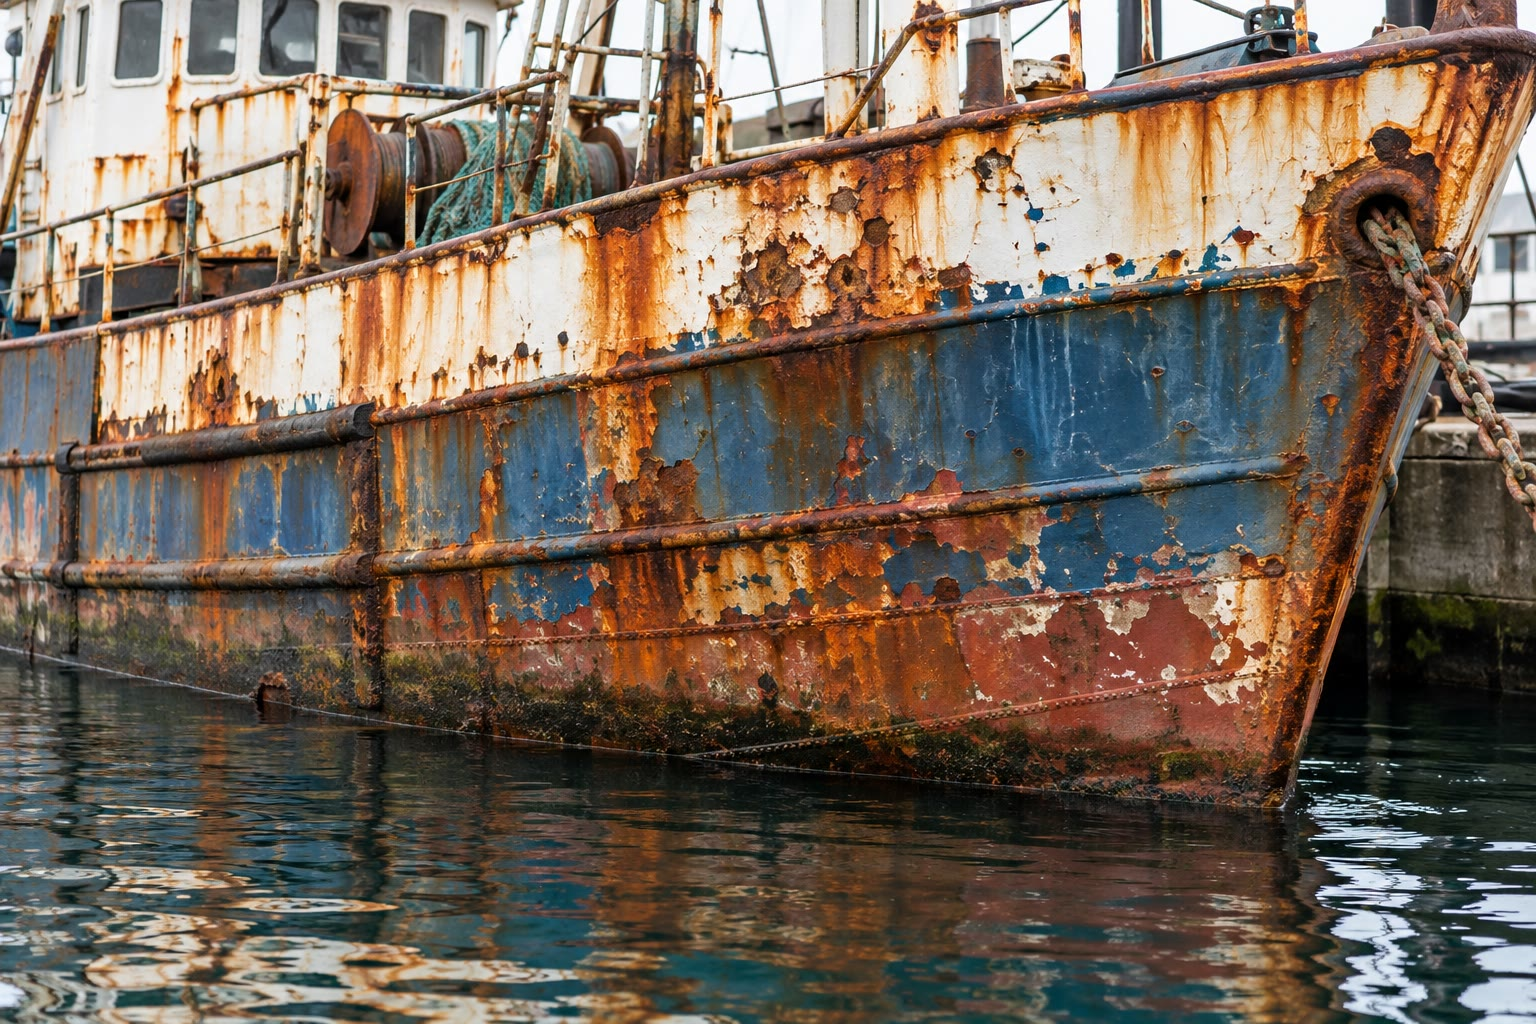
\includegraphics[width=0.55\linewidth]{images/book1/ai/g9-rusty-hull.jpg}

{\small 旧船的船体：钢材正在生锈。}
\end{omfigure}

\section{金属与盐酸}

\begin{inthelab}[三种金属与酸]
老师将少量铁片、锌粒和铜片
分别放入三支盛有稀盐酸的试管中。铁和锌表面冒出气泡，
铁的反应较慢，锌的反应较剧烈，金属逐渐消失；
铜没有任何变化。用小试管收集产生的气体，
点燃时发出“噗”的爆鸣声，说明是氢气。
向第一支试管的液体中加入氢氧化钠溶液，生成绿色\omterm{def:g9:ions:precipitate}{沉淀}（\ce{Fe^{2+}} \omterm{def:g9:ions:ion}{离子}），
第二支试管则生成白色\omterm{def:g9:ions:precipitate}{沉淀}（\ce{Zn^{2+}} \omterm{def:g9:ions:ion}{离子}）。
\end{inthelab}

\begin{omfigure}
\begin{tikzpicture}[font=\small, scale=1.2]
  \foreach \k/\m/\c/\bub in {0/铁/black!45/4, 1/锌/black!25/9, 2/铜/orange!60!brown/0} {
    \pic[transform shape] at (\k*2.4,0) {testtube={0.55}{omWater!70}};
    \fill[\c] (\k*2.4-0.13,0.08) rectangle (\k*2.4+0.13,0.35);
    \ifnum\bub>0
      \foreach \j in {1,...,\bub} {
        \pgfmathsetmacro\yy{0.45+0.12*\j}
        \pgfmathsetmacro\xx{\k*2.4+0.1*sin(97*\j)}
        \draw[black!55] (\xx,\yy) circle (0.035);
      }
    \fi
    \node[anchor=north, align=center] at (\k*2.4,-0.15) {\m};
  }
  \node[anchor=north, align=center, font=\footnotesize] at (0,-0.6) {冒泡，较慢};
  \node[anchor=north, align=center, font=\footnotesize] at (2.4,-0.6) {冒泡，较剧烈};
  \node[anchor=north, align=center, font=\footnotesize] at (4.8,-0.6) {无反应};
\end{tikzpicture}

{\small 铁、锌和铜在稀盐酸中：铁和锌放出氢气；
铜不反应。}
\end{omfigure}

\begin{proposition}[金属与酸的反应]\label{prop:g9:metals-acids-corrosion:acid}
许多金属——如铁、锌、铝、镁——能与酸中的
\ce{H+} \omterm{def:g9:ions:ion}{离子}反应：金属以金属\omterm{def:g9:ions:ion}{离子}的形式消失，这些\omterm{def:g9:ions:ion}{离子}留在溶液中，
同时放出氢气。铜、银和金
不与盐酸反应。
\end{proposition}

\section{用离子写出方程式}

\begin{definition}[旁观离子]\label{def:g9:metals-acids-corrosion:spectator}
在反应过程中存在于溶液中、但不参与反应的\omterm{def:g9:ions:ion}{离子}，
反应结束时仍保持不变，称为\emph{旁观离子}\index{旁观离子}，
写方程式时将其略去。
\end{definition}

\begin{example}[铁和锌与盐酸的反应]\label{ex:g9:metals-acids-corrosion:iron}
盐酸中含有 \ce{H+(aq)} 和 \ce{Cl-(aq)} \omterm{def:g9:ions:ion}{离子}。
氯\omterm{def:g9:ions:ion}{离子}在反应结束时保持不变，它们是\omterm{def:g9:metals-acids-corrosion:spectator}{旁观离子}。
相应的方程式为
\[
  \ce{Fe(s) + 2H+(aq) -> Fe^{2+}(aq) + H2(g)}, \qquad
  \ce{Zn(s) + 2H+(aq) -> Zn^{2+}(aq) + H2(g)}.
\]
两式的\omterm{def:g7:atoms-and-molecules:atom}{原子}与电荷均守恒：两边电荷总数均为 $+2$。
\end{example}

\begin{method}[写出金属与酸反应的方程式]\label{met:g9:metals-acids-corrosion:write}
\begin{enumerate}
  \item \omterm{def:g7:chemical-reactions:reactant}{反应物}：金属 (s) 与 \ce{H+(aq)} \omterm{def:g9:ions:ion}{离子}。
  \item 生成物：带通常电荷的金属\omterm{def:g9:ions:ion}{离子} (aq)，以及
        氢气 \ce{H2(g)}。
  \item 配平\omterm{def:g7:atoms-and-molecules:atom}{原子}，
        然后检查等号两边的总电荷是否相同。
\end{enumerate}
以铝为例：\ce{2Al(s) + 6H+(aq) -> 2Al^{3+}(aq) + 3H2(g)}；
两边电荷均为 $+6$。
\end{method}

\begin{safety}{\ghs[0.8cm]{GHS02}\ghs[0.8cm]{GHS04}}
% ledger: ghs:H2
生成的氢气极易\omterm{def:g4:what-a-fire-needs:burning}{燃烧}。反应
由老师操作，远离明火，
只有爆鸣实验用的火焰除外。
\end{safety}

\section{腐蚀}

\begin{definition}[腐蚀与铁锈]\label{def:g9:metals-acids-corrosion:corrosion}
\emph{腐蚀}\index{腐蚀}是金属缓慢受到周围物质侵蚀的过程，
周围物质（如氧气、水、酸、盐）使金属转变为
\omterm{def:g9:ions:ion}{离子}或氧化物等化合物。铁和钢腐蚀时生成
\emph{铁锈}\index{铁锈}，它是一种棕色、易碎的含水氧化铁，
会剥落，使侵蚀不断向内部深入。
\end{definition}

\begin{proposition}[铁生锈需要什么]\label{prop:g9:metals-acids-corrosion:needs}
铁只有同时接触氧气和水才会生锈。水中\omterm{def:g2:mixing-and-dissolving:dissolve}{溶解}的盐，
如冬季撒过盐的道路上或海边的情况，会使生锈
加快。
\end{proposition}

\begin{inthelab}[三根铁钉，一周]
三根干净的铁钉分别放入三支试管中：第一支装
干燥\omterm{def:g4:air-a-mixture-of-gases:air}{空气}和吸水蒸气的干燥剂；第二支装
煮沸以除去\omterm{def:g2:mixing-and-dissolving:dissolve}{溶解}\omterm{def:g4:air-a-mixture-of-gases:air}{空气}的水，并在水面覆盖一层油；
第三支一半装自来水，一半留有\omterm{def:g4:air-a-mixture-of-gases:air}{空气}。一周后，
只有第三根铁钉生锈。
\end{inthelab}

\begin{omfigure}
\begin{tikzpicture}[font=\small, scale=1.2]
  % tube 1: dry air, drying agent
  \pic[transform shape] at (0,0) {testtube={0.18}{white!80!black}};
  \foreach \x/\y in {-0.12/0.15,0.08/0.12,-0.02/0.3,0.12/0.32,-0.14/0.42,0.03/0.48}
    \fill[black!35] (\x,\y) circle (0.05);
  \fill[black!45] (-0.03,1.0) rectangle (0.03,2.4);
  \fill[black!45] (-0.09,2.4) rectangle (0.09,2.48);
  \fill[black!60] (-0.3,2.8) rectangle (0.3,3.1);
  \node[anchor=north, align=center] at (0,-0.15) {干燥空气：\\ 不生锈};
  % tube 2: boiled water under oil
  \pic[transform shape] at (2.6,0) {testtube={0.7}{omWater!80}};
  \fill[yellow!55!orange!60] (2.36,1.85) rectangle (2.84,2.1);
  \fill[black!45] (2.57,0.3) rectangle (2.63,1.7);
  \fill[black!45] (2.51,1.7) rectangle (2.69,1.78);
  \fill[black!60] (2.3,2.8) rectangle (2.9,3.1);
  \node[anchor=north, align=center] at (2.6,-0.15) {无空气的水：\\ 不生锈};
  % tube 3: water and air
  \pic[transform shape] at (5.2,0) {testtube={0.4}{omWater!80}};
  \fill[black!45] (5.17,0.3) rectangle (5.23,2.2);
  \fill[black!45] (5.11,2.2) rectangle (5.29,2.28);
  \fill[orange!60!brown] (5.15,0.9) rectangle (5.25,1.5);
  \node[anchor=north, align=center] at (5.2,-0.15) {有水有空气：\\ 生锈};
  \draw[<-, omProp, thick] (-0.15,0.3) -- (-0.9,0.7) node[left, text=black, font=\footnotesize] {干燥剂};
  \draw[<-, omProp, thick] (2.85,1.98) -- (3.6,2.4) node[right, text=black, font=\footnotesize] {油};
\end{tikzpicture}

{\small 三根铁钉实验：铁只有在水与氧气同时接触处才生锈，
即图中的水面处。}
\end{omfigure}

\begin{example}[铝和铜自我保护]\label{ex:g9:metals-acids-corrosion:protect}
铝一接触\omterm{def:g4:air-a-mixture-of-gases:air}{空气}中的氧气就会被侵蚀，但生成的薄氧化层
牢牢附着在金属表面，使其与\omterm{def:g4:air-a-mixture-of-gases:air}{空气}隔绝：
铝制窗框可使用数十年。铜会缓慢受到
\omterm{def:g4:air-a-mixture-of-gases:air}{空气}、水和二氧化碳的侵蚀，表面生成一层绿色的膜，
即铜绿，它同样附着牢固，保护下面的金属。相比之下，
\omterm{def:g9:metals-acids-corrosion:corrosion}{铁锈}会剥落。
\end{example}

\begin{omfigure}
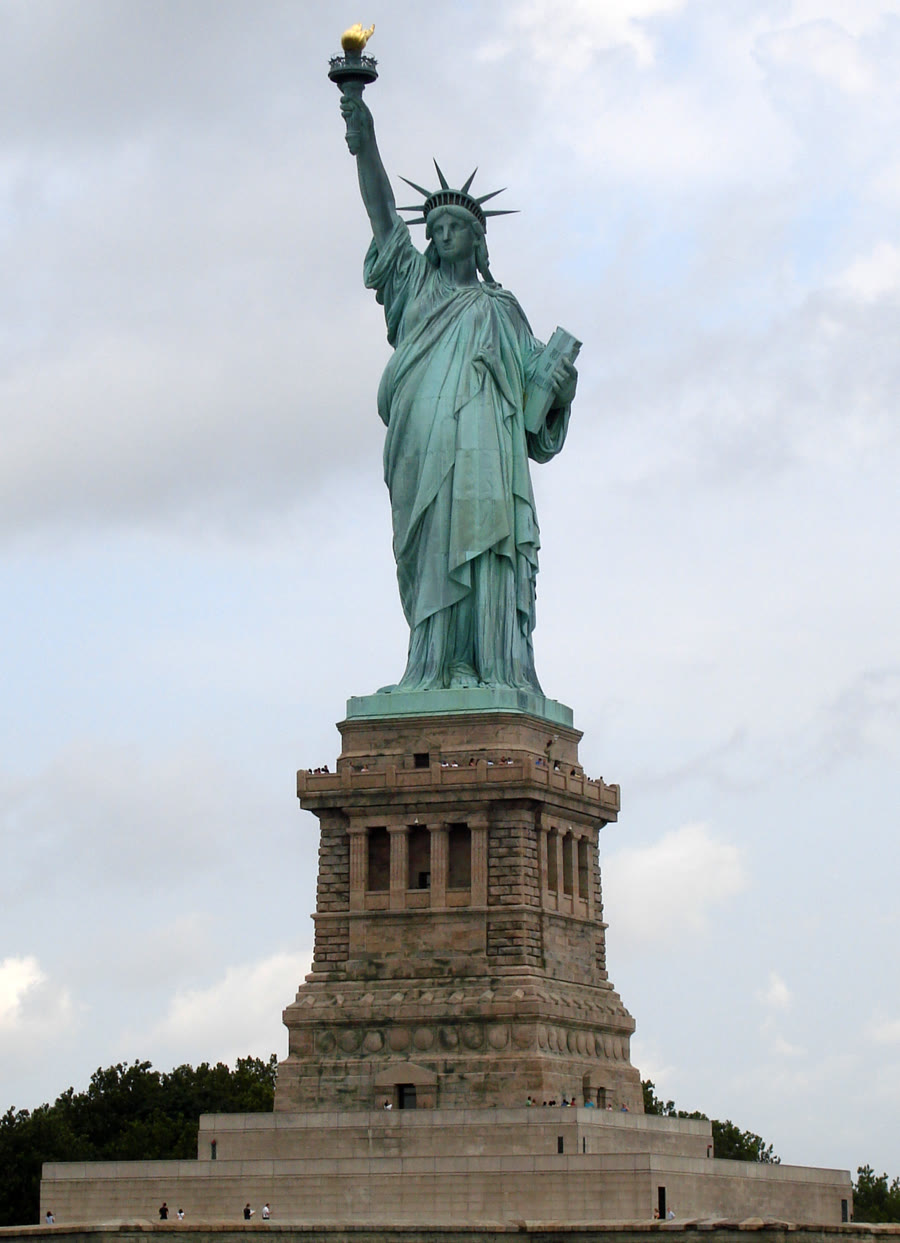
\includegraphics[height=6cm]{images/book1/statue-patina.jpg}

{\small 自由女神像：其铜质表皮覆盖着一层绿色的
铜绿。照片：Elcobbola，公有领域。}
\end{omfigure}

\section{金属的防护}

\begin{definition}[镀锌]\label{def:g9:metals-acids-corrosion:galvanising}
\emph{镀锌}\index{镀锌}是通过将钢材浸入熔融的锌中，使其表面
覆盖一层锌。锌被\omterm{def:g4:air-a-mixture-of-gases:air}{空气}和水侵蚀，而不是下面的钢；
即使镀层被划伤，
附近的锌会先被\omterm{def:g9:metals-acids-corrosion:corrosion}{腐蚀}，钢材得以保护。
\end{definition}

\begin{proposition}[铁和钢的防护方法]\label{prop:g9:metals-acids-corrosion:ways}
\begin{itemize}
  \item 隔绝水和\omterm{def:g4:air-a-mixture-of-gases:air}{空气}：涂漆、涂油、涂润滑脂、覆盖\omterm{def:g8:plastics:plastic}{塑料}膜；
  \item \omterm{def:g9:metals-acids-corrosion:galvanising}{镀锌}：用锌层代替钢材发生\omterm{def:g9:metals-acids-corrosion:corrosion}{腐蚀}；
  \item 使用不锈钢，即铁与铬的合金，它
        借助一层薄而致密的氧化膜保护自身；
  \item 在船体上固定锌块：锌块代替钢材被缓慢消耗，
        并定期更换（其原理
        将在大学教材中讲解）。
\end{itemize}
\end{proposition}

\begin{omfigure}
\begin{minipage}[b]{0.52\linewidth}\centering
\begin{tikzpicture}[font=\small]
  \fill[black!35] (0,0) rectangle (5,0.8);
  \fill[black!15] (0,0.8) rectangle (2.2,1.1);
  \fill[black!15] (2.8,0.8) rectangle (5,1.1);
  \fill[omWater!80] (1.6,1.1) rectangle (3.4,1.35);
  \fill[omWater!80] (2.2,0.8) rectangle (2.8,1.1);
  \draw[black!60] (0,0) rectangle (5,0.8);
  \foreach \x in {1.95,2.1} \draw[->, omProp, thick] (\x,1.25) -- (\x+0.05,1.7);
  \node[anchor=west, font=\footnotesize] at (5.1,0.4) {钢};
  \node[anchor=west, font=\footnotesize] at (5.1,0.95) {锌层};
  \node[anchor=south, font=\footnotesize, align=center] at (2.0,1.75) {锌离子 \\ 进入水中};
  \node[anchor=north, font=\footnotesize, align=center] at (2.5,-0.05) {划痕处：钢材 \\ 暴露，周围的锌 \\ 先被腐蚀};
\end{tikzpicture}

{\small 划痕后的\omterm{def:g9:metals-acids-corrosion:galvanising}{镀锌}板。}
\end{minipage}\hfill
\begin{minipage}[b]{0.44\linewidth}\centering
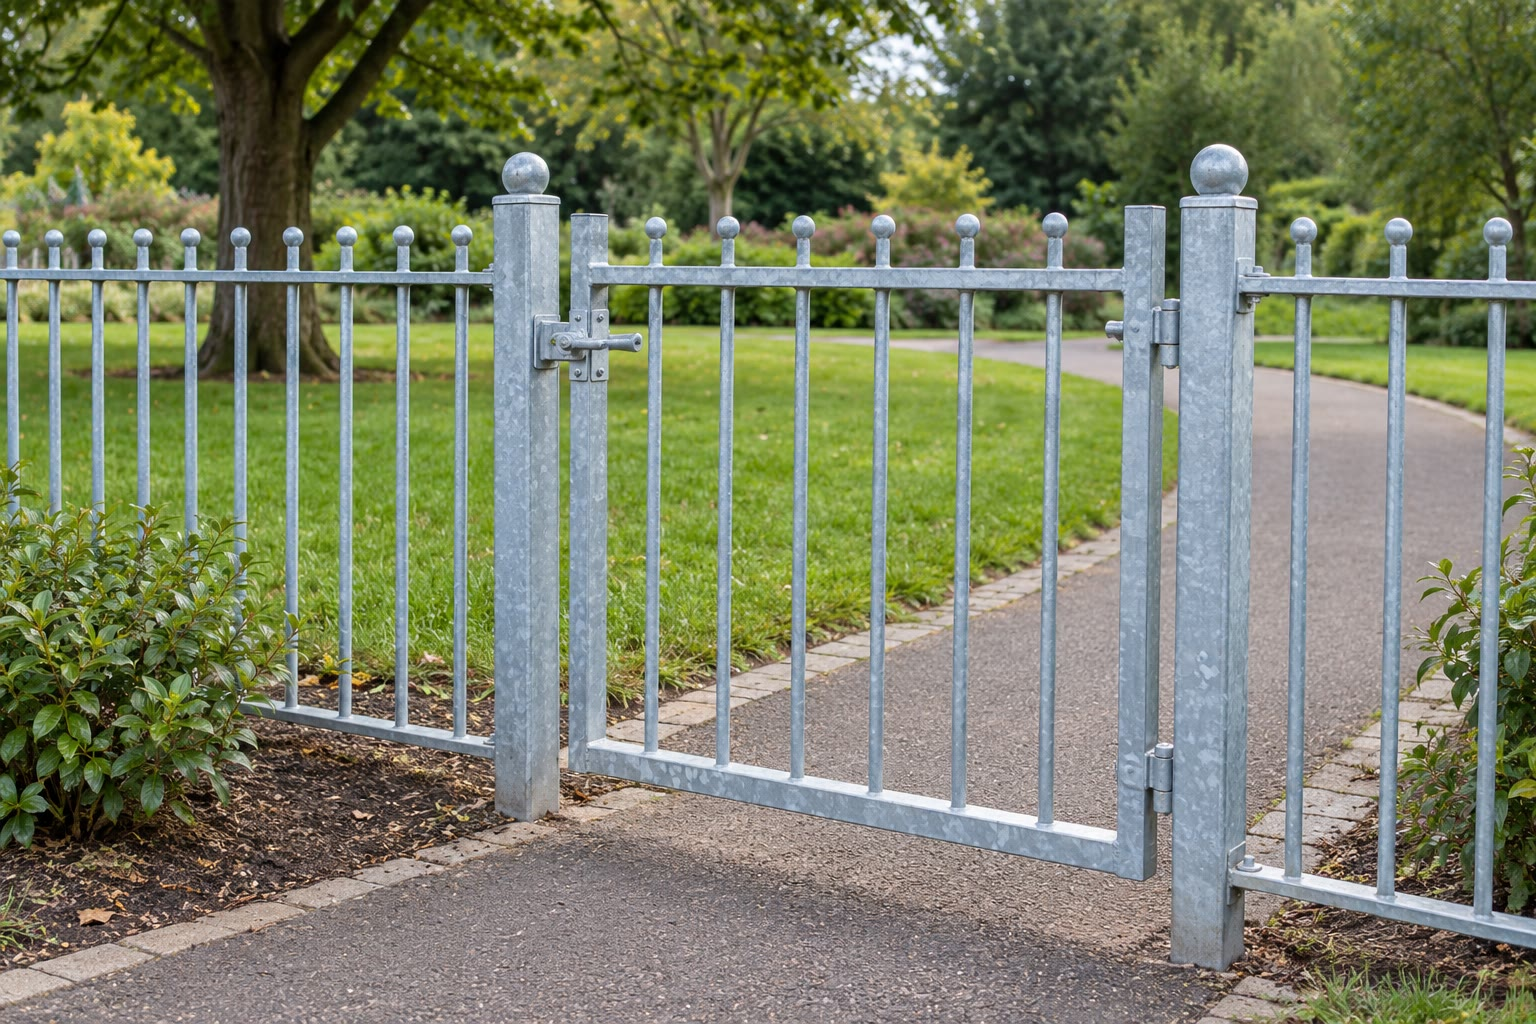
\includegraphics[width=\linewidth,height=4.4cm,keepaspectratio]{images/book1/ai/g9-galvanised-railings.jpg}

{\small \omterm{def:g9:metals-acids-corrosion:galvanising}{镀锌}钢栏杆。}
\end{minipage}
\end{omfigure}

\section{练习}

\begin{exercise}[$\star$]\label{exo:g9:metals-acids-corrosion:1}
锌与盐酸反应时放出哪种气体？
如何检验该气体？
\end{exercise}

\begin{exercise}[$\star$]\label{exo:g9:metals-acids-corrosion:2}
下列哪些金属能与稀盐酸反应：铁、铜、
锌、金、铝？
\end{exercise}

\begin{exercise}[$\star$]\label{exo:g9:metals-acids-corrosion:3}
铁生锈需要什么条件？
\end{exercise}

\begin{exercise}[$\star$]\label{exo:g9:metals-acids-corrosion:4}
什么是\omterm{def:g9:metals-acids-corrosion:spectator}{旁观离子}？指出铁与
盐酸反应时的\omterm{def:g9:metals-acids-corrosion:spectator}{旁观离子}。
\end{exercise}

\begin{exercise}[$\star\star$]\label{exo:g9:metals-acids-corrosion:5}
写出镁与酸中的 \ce{H+} \omterm{def:g9:ions:ion}{离子}反应
的方程式（镁\omterm{def:g9:ions:ion}{离子}为 \ce{Mg^{2+}}）。检查电荷是否守恒。
\end{exercise}

\begin{exercise}[$\star\star$]\label{exo:g9:metals-acids-corrosion:6}
铁与盐酸反应后，如何证明
溶液中是否含有亚铁\omterm{def:g9:ions:ion}{离子}？
\end{exercise}

\begin{exercise}[$\star\star$]\label{exo:g9:metals-acids-corrosion:7}
观察三钉实验图。为什么第二支试管中的水
要煮沸并用油覆盖？
\end{exercise}

\begin{exercise}[$\star\star$]\label{exo:g9:metals-acids-corrosion:8}
为什么在冬季撒盐融雪的城市里，汽车生锈更快？
\end{exercise}

\begin{exercise}[$\star\star$]\label{exo:g9:metals-acids-corrosion:9}
为什么铝制窗框不会锈蚀殆尽，
尽管铝能与\omterm{def:g4:air-a-mixture-of-gases:air}{空气}中的氧气反应？
\end{exercise}

\begin{exercise}[$\star\star$]\label{exo:g9:metals-acids-corrosion:10}
给出保护钢制自行车车架防锈的三种方法。
\end{exercise}

\begin{exercise}[$\star\star\star$]\label{exo:g9:metals-acids-corrosion:11}
写出并检查铝与酸中的
\ce{H+} \omterm{def:g9:ions:ion}{离子}反应的方程式。求 200 个
铝\omterm{def:g7:atoms-and-molecules:atom}{原子}可生成多少个氢\omterm{def:g7:atoms-and-molecules:molecule}{分子}？
\end{exercise}

\begin{exercise}[$\star\star\star$]\label{exo:g9:metals-acids-corrosion:12}
一只\omterm{def:g9:metals-acids-corrosion:galvanising}{镀锌}钢桶的表面被刮出一道伤痕，直至露出钢。试说明
伤痕底部的钢为何长时间不生锈。
\end{exercise}

\section{问题：锌层有多厚？}

\begin{problem}[{周末问题——溶解镀锌钢板的
锌层，以求其厚度}]
\label{pb:g9:metals-acids-corrosion:1}
% ledger: rho:Zn
一块\omterm{def:g9:metals-acids-corrosion:galvanising}{镀锌}钢板为边长 \qty{10.0}{cm} 的正方形，两面均
镀有锌层（忽略边缘）。在实验室中，教师
先将其称得 \qty{125.6}{g}，然后将其浸入含有
一种添加剂的盐酸中，该添加剂可阻止酸\omterm{def:g9:metals-acids-corrosion:corrosion}{腐蚀}钢。待气泡
停止冒出后，将钢板冲洗、晾干并再次称量，质量为 \qty{113.5}{g}。
已知 \qty{1}{cm^3} 锌的质量为 \qty{7.13}{g}。

\medskip
\noindent\textbf{第一部分——反应。}
\begin{enumerate}
  \item 写出锌与酸中的 \ce{H+} \omterm{def:g9:ions:ion}{离子}
        反应的方程式。
  \item 哪种气体引起气泡？描述其检验方法。
  \item 用哪种检验方法可证明反应后溶液中含有锌\omterm{def:g9:ions:ion}{离子}？
  \item 指出\omterm{def:g9:metals-acids-corrosion:spectator}{旁观离子}。
\end{enumerate}

\medskip
\noindent\textbf{第二部分——锌。}
\begin{enumerate}[resume]
  \item 已\omterm{def:g2:mixing-and-dissolving:dissolve}{溶解}的锌的质量为多少？
  \item 为什么仍有气泡冒出，说明锌
        尚未全部\omterm{def:g2:mixing-and-dissolving:dissolve}{溶解}？
  \item 若酸中不含该添加剂，钢会发生什么
        变化？用哪种检验方法证实？
  \item 只要锌层尚存，锌为什么能保护
        钢板？
\end{enumerate}

\medskip
\noindent\textbf{第三部分——厚度。}
\begin{enumerate}[resume]
  \item 钢板镀层的总面积为多少 \unit{cm^2}？
  \item 锌所占的体积为多少？
  \item 推算锌层的厚度，单位为厘米。
  \item 将该厚度换算为微米。
        (\qty{1}{cm} $= \qty{10000}{\micro m}$).
\end{enumerate}
\end{problem}
